\documentclass{article}
%\usepackage{style}
\usepackage[ruled, algo2e]{algorithm2e}
\usepackage{amsmath, amsfonts, amsthm}

%\usepackage{graphicx, epstopdf}
\usepackage{color}
\usepackage{cite}
\usepackage{indentfirst}
\usepackage{geometry, graphicx}
\usepackage[title]{appendix}
\usepackage{algorithm, algorithmic}
\usepackage{bm}
\usepackage[hidelinks]{hyperref}
\usepackage{multirow}
\usepackage[tight]{subfigure}
%\usepackage{ulem}
\geometry{left = 5em, right = 5em}
\usepackage{listings}
\usepackage{xcolor}
\usepackage{subfigure} 
%% notation macro
\newcommand{\OB}{\Ocal\B}
\newcommand{\Rt}{\operatorname{Rt}}
\newcommand{\Grad}{\operatorname{grad}}
\newcommand{\sign}{\operatorname{sign}}
\newcommand{\diag}{\operatorname{diag}}
\newcommand{\tfo}{\textbf{1}}
\newcommand{\E}{\mathcal E}
\newcommand{\F}{\mathcal F}
\newcommand{\T}{\mathcal T}
\newcommand{\I}{\mathcal I}
\newcommand{\Ocal}{\mathcal O}
\newcommand{\Ibf}{\mathbf I}
\newcommand{\Y}{\mathcal Y}
\newcommand{\Ybf}{\mathbf Y}
% \newcommand{\U}{\mathcal U}
\newcommand{\R}{\mathbb R}
\renewcommand{\P}{\mathcal P}
\newcommand{\uP}{ \mathcal \uline P}
\newcommand{\V}{\mathcal V}
\newcommand{\A}{\mathcal A}
\newcommand{\B}{\mathcal B}
\newcommand{\G}{\mathcal G}
\newcommand{\Hcal}{\mathcal Hcal}
%\newcommand{\R}{\mathbb R^2}
\newcommand{\Z}{\mathbb Z}
\newcommand{\Eb}{\mathbb E}
% \newcommand{\C}{\mathbb C}
\newcommand{\laplacian}{\triangle}
\newcommand{\grad}{\nabla}
\renewcommand{\div}{\textrm{div~}}
% cf
\newcommand{\iprod}[2]{\left\langle #1, #2 \right\rangle}
\newcommand{\II}[1]{\mathbb{1}\left\{#1\right\}}
\newcommand{\nrm}[1]{\left\|#1\right\|}
\newcommand{\bH}{\mathbf{H}}
\newcommand{\eps}{\varepsilon}
\newcommand{\DD}{\mathbb{D}}
\newcommand{\RR}{\mathbb{R}}
\newcommand{\cO}{\mathcal{O}}
\newcommand{\cB}{\mathcal{B}}
\newcommand{\PP}{\mathbb{P}}
\newcommand{\EE}{\mathbb{E}}
\newcommand{\relu}{\operatorname{ReLU}}
\renewcommand{\II}[1]{\mathbb{I}\left\{#1\right\}\}}

\newcommand{\diff}[2]{\frac{\partial #1}{\partial #2}}
\newcommand{\difff}[3]{\frac{\parial #1^2}{\partial #2 \partial #3}}
\newcommand{\diFF}[2]{\frac{\partial #1^2}{\partial^2 #2}}
\newcommand{\diam}{\text{ diam }}
%% non-noation macro
\newcommand{\IN}{\text{  in  }}
\newcommand{\ON}{\text{  on  }}
\newcommand{\st}{\text{s.t.  }}
\newcommand{\tbc}{{\color{red}[TBC]}}
\newcommand\ldq\textquotedblleft
\newcommand\rdq\textquotedblright{}
\newcommand\mb\mathbb
\newcommand\mf\mathbf
\newcommand\tf\textbf
\newcommand{\revise}[1]{{\color{blue}#1}}

\newcommand{\return}{\textbf{return~}}
\DeclareMathOperator{\argmin}{arg~min}
\DeclareMathOperator{\argmax}{arg~max}
%% enviorment
\newtheorem{proposition}{Proposition}
\newtheorem{definition}{Definition}
\newtheorem{corollary}{Corollary}
\newtheorem{remark}{Remark}
\newtheorem{assumption}{Assumption}
\newtheorem{Proposition}{Proposition}
\newtheorem{Definition}{Definition}
\newtheorem{Corollary}{Corollary}
\newtheorem{Remark}{Remark}
\newtheorem{Assumption}{Assumption}
\newtheorem{Condition}{Condition}
\newtheorem{condition}{Condition}
\newtheorem{theorem}{Theorem}
\newtheorem{lemma}{Lemma}
\setlength{\parindent}{1.5em}
\definecolor{mygreen}{rgb}{0,0.6,0}
\definecolor{mygray}{rgb}{0.5,0.5,0.5}
\definecolor{mymauve}{rgb}{0.58,0,0.82}
\lstset{ %
	backgroundcolor=\color{white},      % choose the background color
	basicstyle=\footnotesize\ttfamily,  % size of fonts used for the code
	columns=fullflexible,
	tabsize=4,
	breaklines=true,               % automatic line breaking only at whitespace
	captionpos=b,                  % sets the caption-position to bottom
	commentstyle=\color{green},  % comment style
	escapeinside={\%*}{*)},        % if you want to add LaTeX within your code
	keywordstyle=\color{blue},     % keyword style
	stringstyle=\color{mymauve}\ttfamily,  % string literal style
	frame=single,
	rulesepcolor=\color{red!20!green!20!blue!20},
	% identifierstyle=\color{red},
	language=matlab,
	numbers=left,
}
\title{\textbf{\showtitle}}
\author{\showauthor}
\usepackage{indentfirst}
\usepackage{fancyhdr}  
\pagestyle{fancy}

\renewcommand{\algorithmicrequire}{\textbf{Input}}
\renewcommand{\algorithmicensure}{\textbf{Output}}
%\lhead{\textbf {\showtopic} }
%\chead{} 
%\rhead{\textbf {\showabs} }
%\lfoot{} 
%\cfoot{\thepage}
%\rfoot{} 
%\renewcommand{\headrulewidth}{0.4pt} 
%\usepackage{lineno}
%\linenumbers
\usepackage{caption}

\newcommand{\be}{\begin{equation}}
\newcommand{\ee}{\end{equation}}
\newcommand{\mL}{\mathcal L}
\newcommand{\dA}{\Delta(\A)}
\newcommand{\dB}{\Delta(\B)}
\newcommand{\KL}{\mathrm{KL}}
\newcommand{\dualgap}{\Operatorname{DualGap}}
\newcommand{\prox}{\mathrm{prox}}
\newcommand{\proj}{\mathrm{proj}}
\title{Phase Retrieval}
\date{\today}	
\author{Ruicheng Ao 1900012179}
\begin{document}
\maketitle
\section{Problem description}
One popular formulation of the phase retrieval problem is solving a system of quadratic equations in the form
\begin{equation}
	y_i = |\langle a_i,z\rangle|^2,i=1,2,\dots,m,
\end{equation}
where $z\in\Ccal^n$ is the decision variable, $a_i\in\Ccal^n$ are known sampling vectors, $\langle a_i,z\rangle$ is the inner product between $a_i$ and $z$, $|\cdot|$ denotes the norm and $y_i\in\R$ are the observed measurements. The relationship can be reformulated into minimal square error problem 
\begin{equation}\label{prob}
	\begin{array}{cc}
		\min_{z\in\Ccal^n} & f(z)=\frac{1}{2m}\sum_{r=1}^m(|\langle a_r,z\rangle|^2-y_r)^2.
	\end{array}
\end{equation}
In this report, we mainly focus on the algorithm, which starts with a careful initialization obtained by means of eigenvector and iteratively applies novel update rules proposed in \cite{candes2015phase} that solves the problem \eqref{prob} efficiently.
\section{Algorithm description}
The algorithm chooses carefully the initial point $z^0$ via a spectral method so that the iterates $\{z^t\}_{t=0}^\infty$ converge to the solution with high probability. To speak more specifically, $z^0$ is chosen as the leading eigenvector of the positive definite Hermitian matrix $\sum_{r=1}^my_ra_ra_r^*$. The framework is given in Algorithm \ref{alg1}.
\begin{algorithm}[H]
	\caption{Wirtinger Flow: Initialization}
	\begin{algorithmic}[1]\label{alg1}
		\REQUIRE{Observation $A=[a_1,a_2,\dots,a_m]\in\Ccal^{n\times m},y=[y_1,y_2,\dots,y_m]\in\R^m$, the number of iterations $T$}
		\STATE{Set $\lambda = \min\{\sqrt{n\frac{\sum_{r=1}^my_r}{\sum_{r=1}^m\|a_r\|_2^2}},\sqrt{\frac{\sum_{r=1}^my_r}{\operatorname{numel}(y)}}\}$}
		\FOR{$t=1,2,\dots,T$}
		\STATE{Update $z^0 = A\diag(y)A^*z^0$}
		\STATE{Normalize $z^0= z^0/\|z^0\|_2^2$}
		\ENDFOR
		\STATE{Normalize $z^0 = \lambda z^0$}
		\RETURN{$z^0$}
	\end{algorithmic}
\end{algorithm}

After initializing the iterate $z^0$, a vanilla gradient descent method is applied in \cite{candes2015phase}, namely,
\begin{equation}
	\begin{aligned}
		z^{t+1} &= z^t - \frac{\mu_t}{\|z^0\|^2}\nabla f(z^t)\\
		&= z^t - \frac{\mu_t}{\|z^0\|^2}(\frac{1}{m}\sum_{r=1}^m(|a_r^*z|-y_r)a_ra_r^*z),
	\end{aligned}
\end{equation}
which is a form of steepest descent and the parameter $\mu_t$ is the step size. Note nonetheless that the feective step size is inversely proportional to the magnitude of the initial guess.
\section{Numerical experiments}
We test the introduced algorithm on two datasets for 1D Wirtinger Flow in \cite{candes2015phase}, namely, Gaussian dataset and coded diffraction patterns (CDP) dataset to show the efficiency. For Gaussian dataset, we test the case when $n=64,128,256$ and $m=400,800,1200$. For CDP dataset, we choose $L=3,6,12$ and $n=128,256,512$. The step size is chosen to be $\mu_t = \min\{\mu,\exp(-t/\tau_0)\},$ where $\tau$ is selected from the set $\{0.02,0.05,0.1,0.2,0.3\}$ for comparison and $\tau_0 = 330$. The number of power iterations in initialization is selected to be $50$ as the same as \cite{candes2015phase}. The numerical results are shown as below. Table \ref{gaussian} and \ref{CDP} give the relative error in $\ell_2$ norm with the primitive data after $3000$ iterations. Figures 1-18 display the iterative curves on different datasets and parameters.
\begin{table}
	\centering
	\begin{tabular}{|c|c|c|c|c|c|}
	\hline
	\multirow{2}{*}{ $\mu$} &\multicolumn{5}{c|}{$n = 64 $}\\\cline{2-6}
	 &$0.02$ &$0.05$ &$0.1$ &$0.2$ &$0.3$\\\hline
	$m=400$ & $5.79e-05$ & $6.86e-10$ & $2.22e-15$ & $3.63e-16$ & $2.53e-16$\\\hline
	$m=800$ & $1.70e-04$ & $3.37e-09$ & $2.34e-15$ & $4.52e-16$ & $2.80e-16$\\\hline
	$m=1200$ & $3.57e-05$ & $4.36e-10$ & $2.52e-15$ & $3.22e-16$ & $3.12e-16$\\\hline
	\multirow{2}{*}{ $\mu$} &\multicolumn{5}{c|}{$n = 256 $}\\\cline{2-6}
	&$0.02$ &$0.05$ &$0.1$ &$0.2$ &$0.3$\\\hline
	$m=400$ & $1.55e-04$ & $5.48e-09$ & $2.49e-15$ & $4.42e-16$ & $3.71e-16$\\\hline
	$m=800$ & $5.77e-05$ & $9.52e-10$ & $1.92e-15$ & $3.69e-16$ & $3.94e-16$\\\hline
	$m=1200$ & $1.13e+00$ & $1.14e+00$ & $1.14e+00$ & $1.14e+00$ & $1.14e+00$\\\hline
	\multirow{2}{*}{ $\mu$} &\multicolumn{5}{c|}{$n = 256 $}\\\cline{2-6}
 &$0.02$ &$0.05$ &$0.1$ &$0.2$ &$0.3$\\\hline
$m=400$ & $6.08e-02$ & $9.47e-05$ & $2.05e-09$ & $8.84e-16$ & $5.35e-16$\\\hline
$m=800$ & $3.24e-03$ & $8.42e-06$ & $1.11e-09$ & $6.04e-16$ & $4.85e-16$\\\hline
$m=1200$ & $1.85e-03$ & $4.58e-06$ & $3.66e-10$ & $6.12e-16$ & $4.89e-16$\\\hline
	\end{tabular}
	\caption{Relative error after $3000$ iterations by Wirtinger Flow on dataset Gaussian\label{gaussian}}
	\end{table}
	\begin{figure}
		\begin{minipage}{0.33\linewidth}
			\centering
			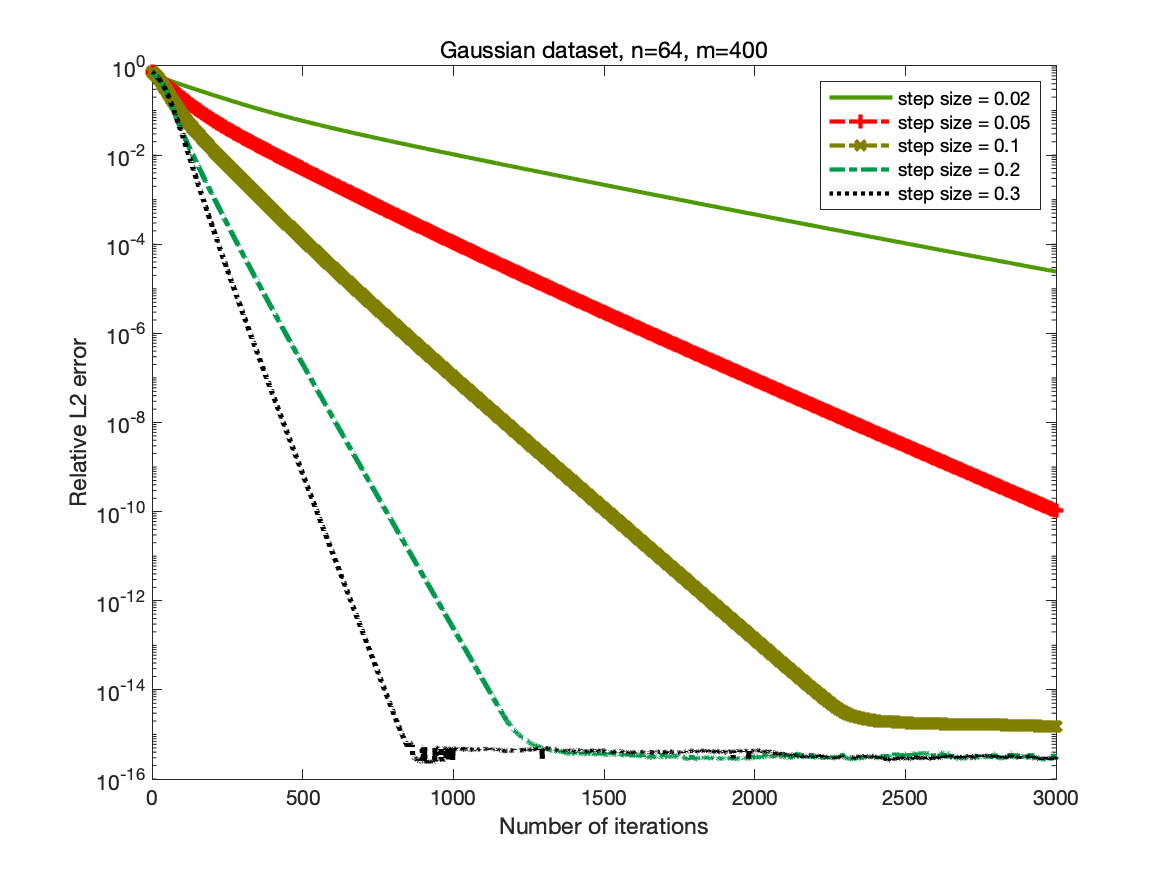
\includegraphics[width=1\linewidth]{./fig/gaussian+11.png}
			\caption{$m=400$}
		\end{minipage}
		\begin{minipage}{0.33\linewidth}
			\centering
			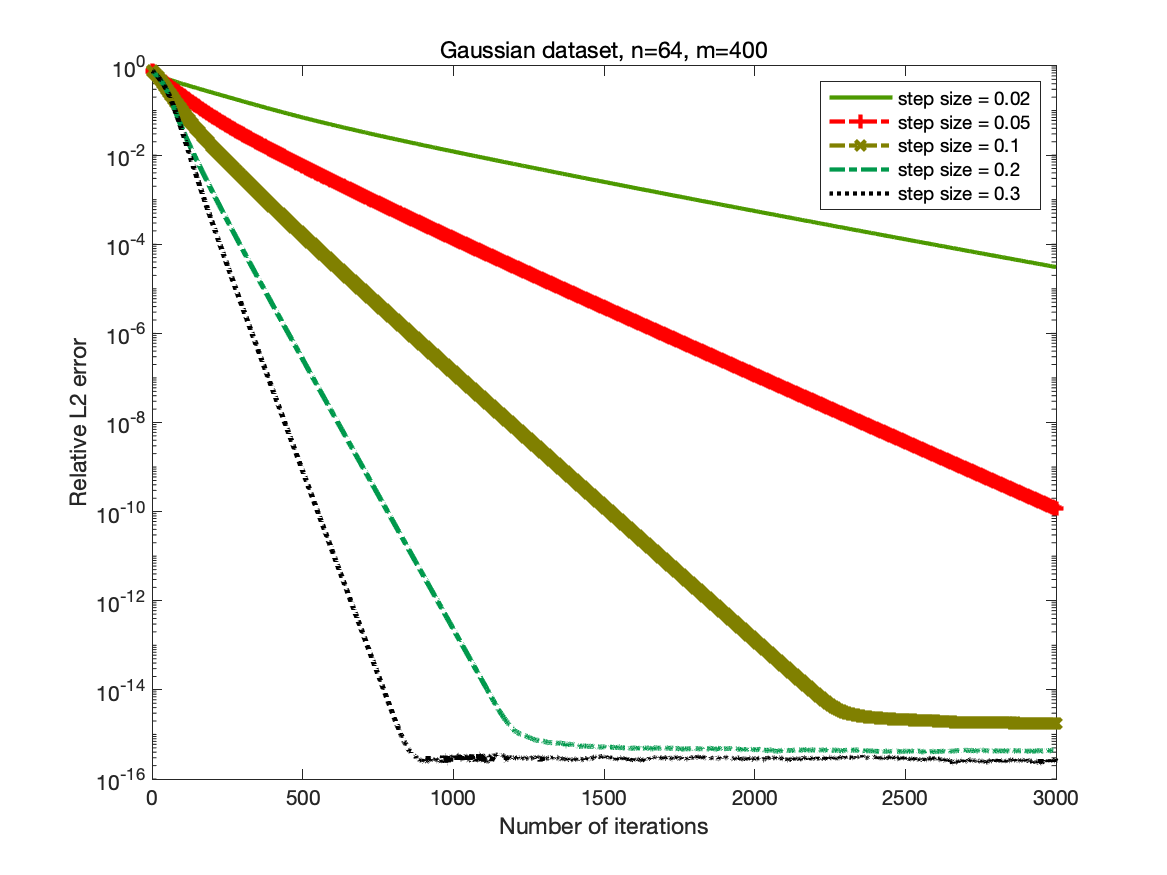
\includegraphics[width=1\linewidth]{./fig/gaussian+12.png}
			\caption{$m=800$}
		\end{minipage}
		\begin{minipage}{0.33\linewidth}
			\centering
			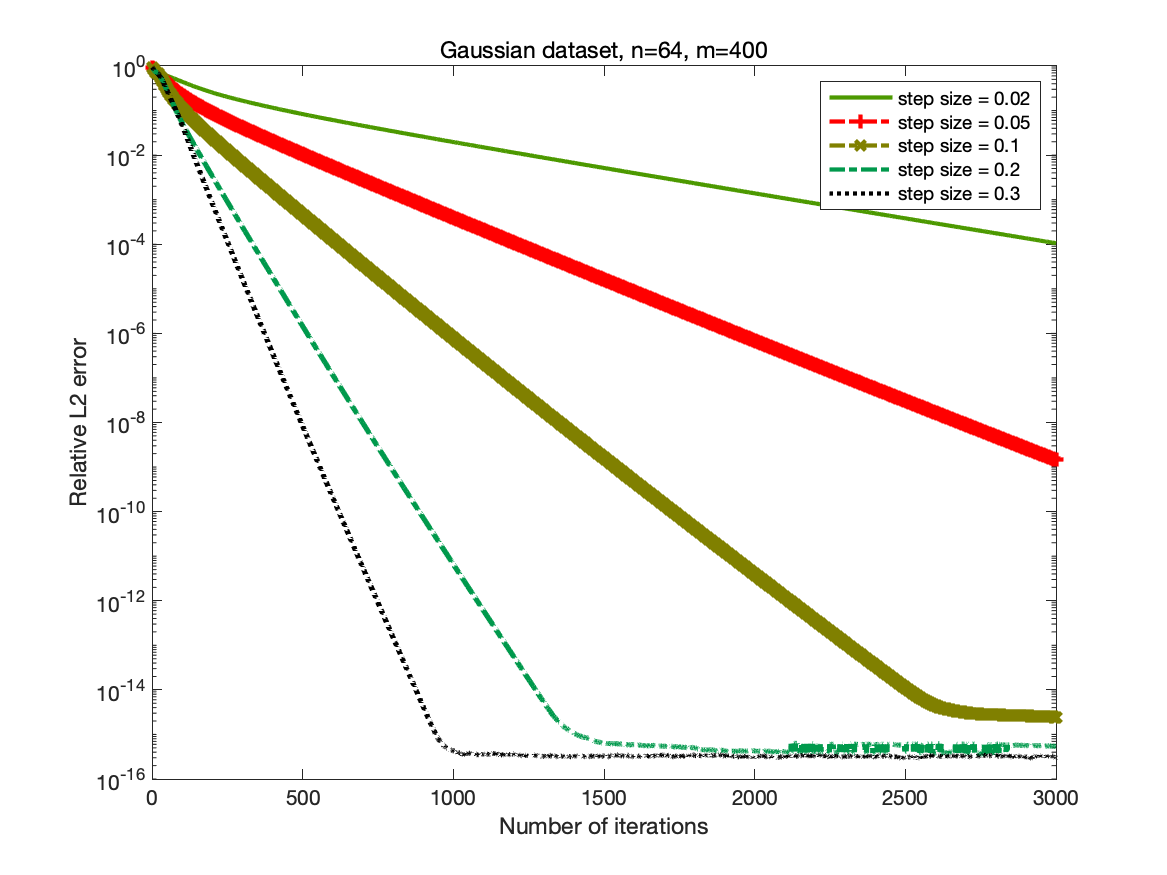
\includegraphics[width=1\linewidth]{./fig/gaussian+13.png}
			\caption{$m=1200$}
		\end{minipage}
		\caption*{Results on Gaussian dataset when $n=64$}
	\end{figure}
	\begin{figure}
		\begin{minipage}{0.33\linewidth}
			\centering
			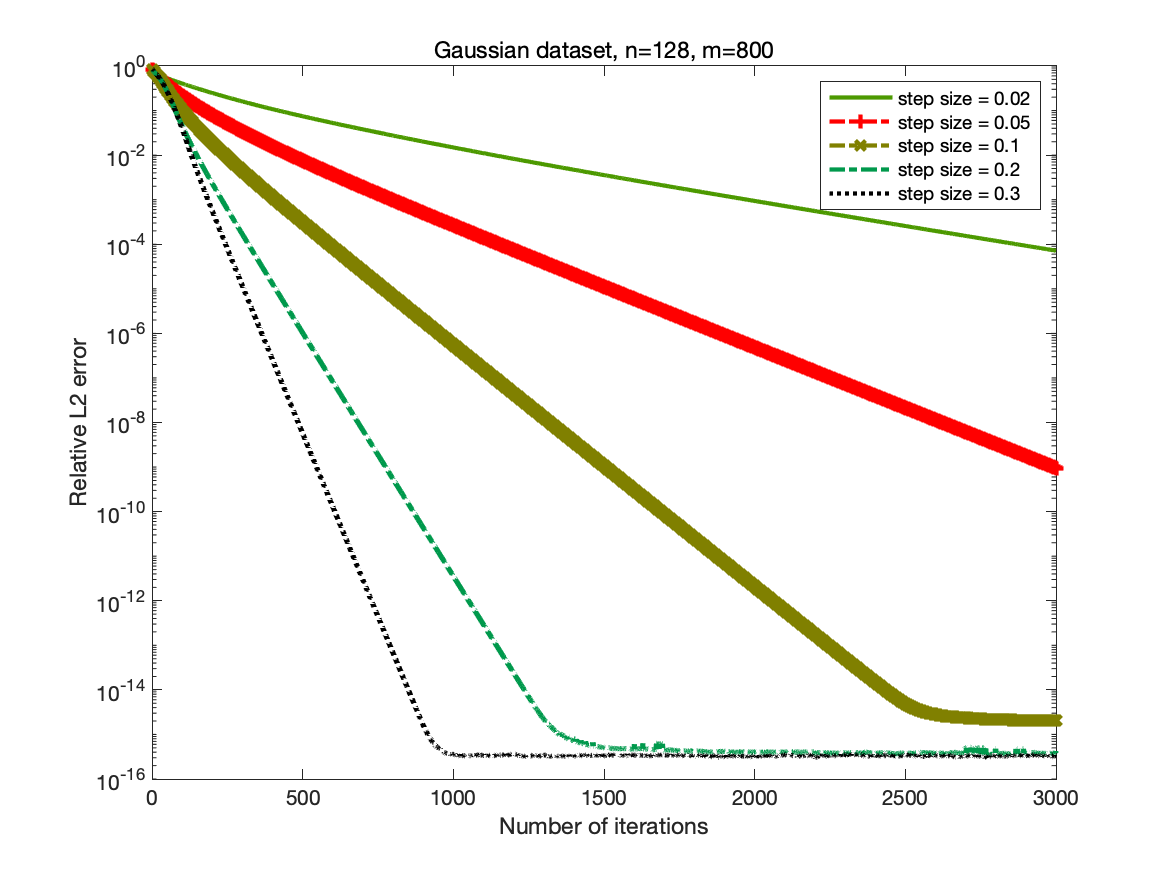
\includegraphics[width=1\linewidth]{./fig/gaussian+21.png}
			\caption{$m=400$}
		\end{minipage}
		\begin{minipage}{0.33\linewidth}
			\centering
			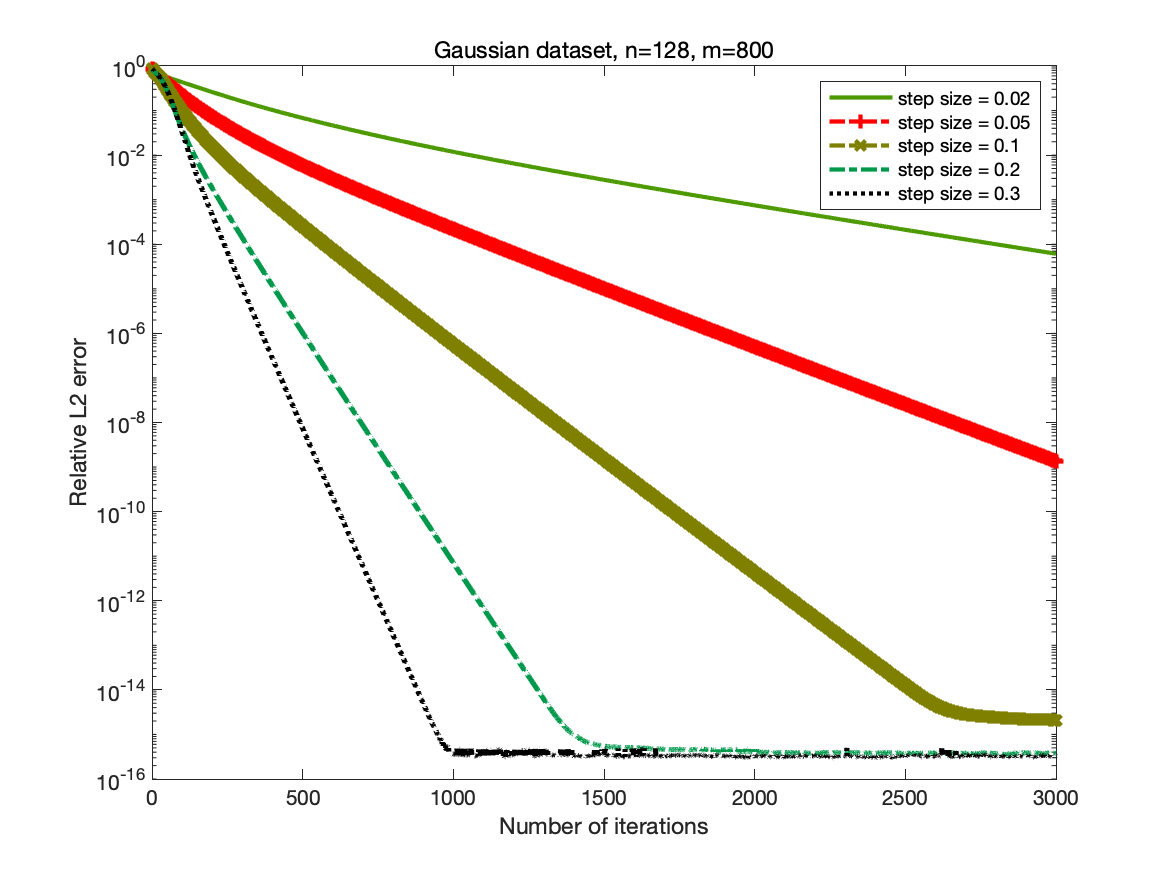
\includegraphics[width=1\linewidth]{./fig/gaussian+22.png}
			\caption{$m=800$}
		\end{minipage}
		\begin{minipage}{0.33\linewidth}
			\centering
			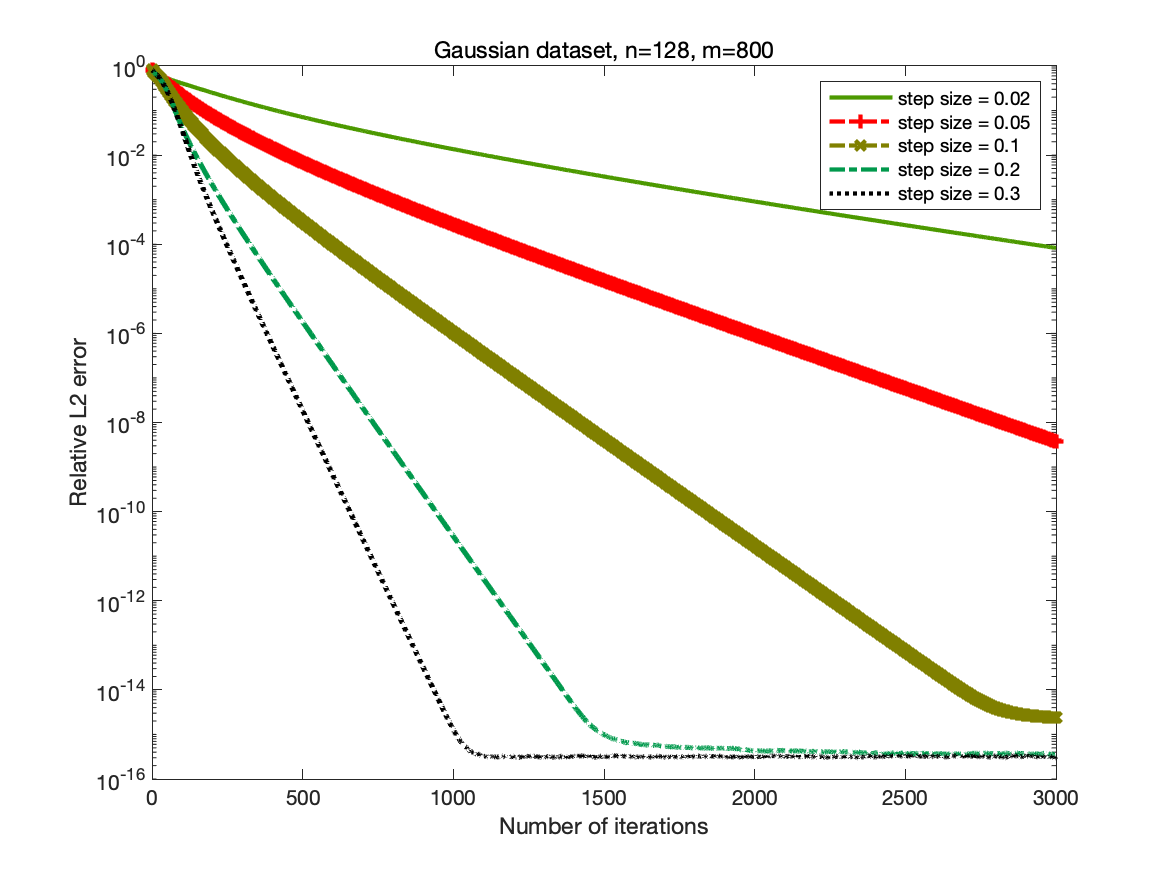
\includegraphics[width=1\linewidth]{./fig/gaussian+23.png}
			\caption{$m=1200$}
		\end{minipage}
		\caption*{Results on Gaussian dataset when $n=128$}
	\end{figure}
	\begin{figure}
		\begin{minipage}{0.33\linewidth}
			\centering
			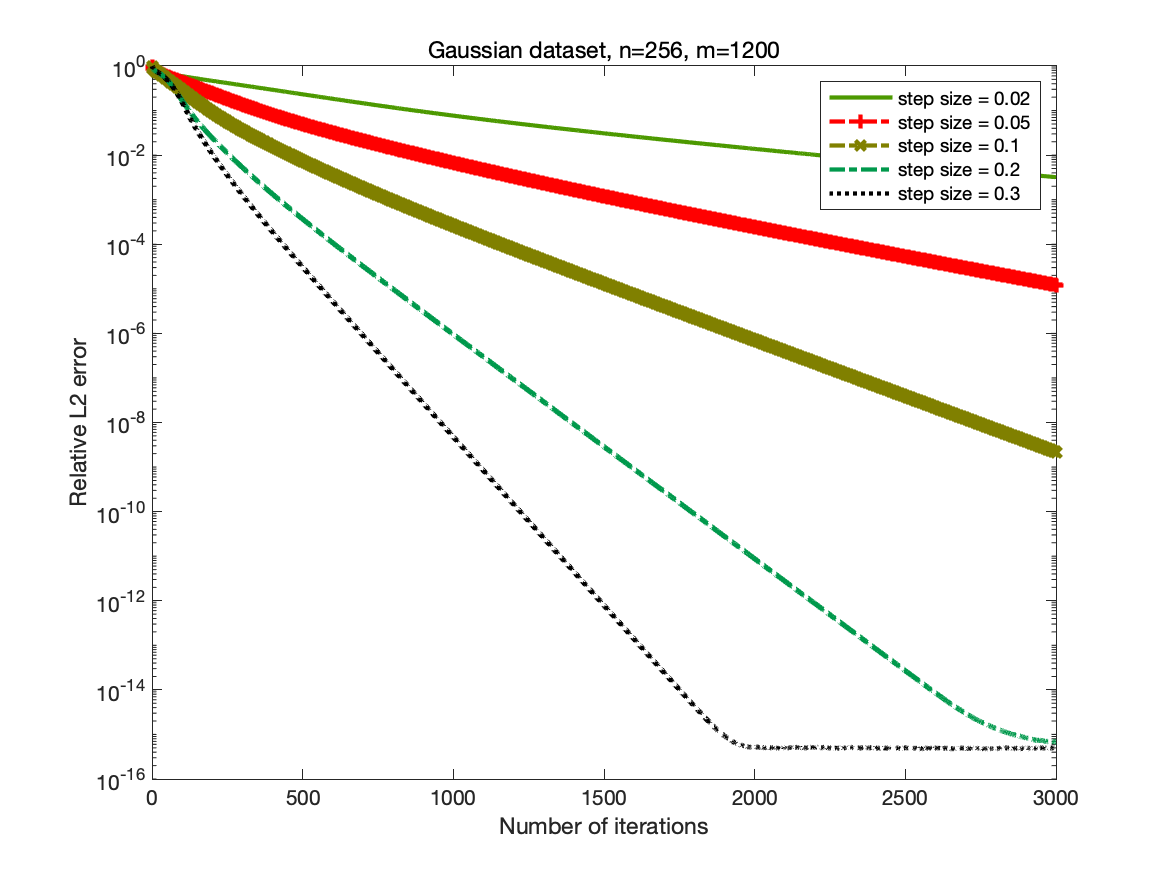
\includegraphics[width=1\linewidth]{./fig/gaussian+31.png}
			\caption{$m=400$}
		\end{minipage}
		\begin{minipage}{0.33\linewidth}
			\centering
			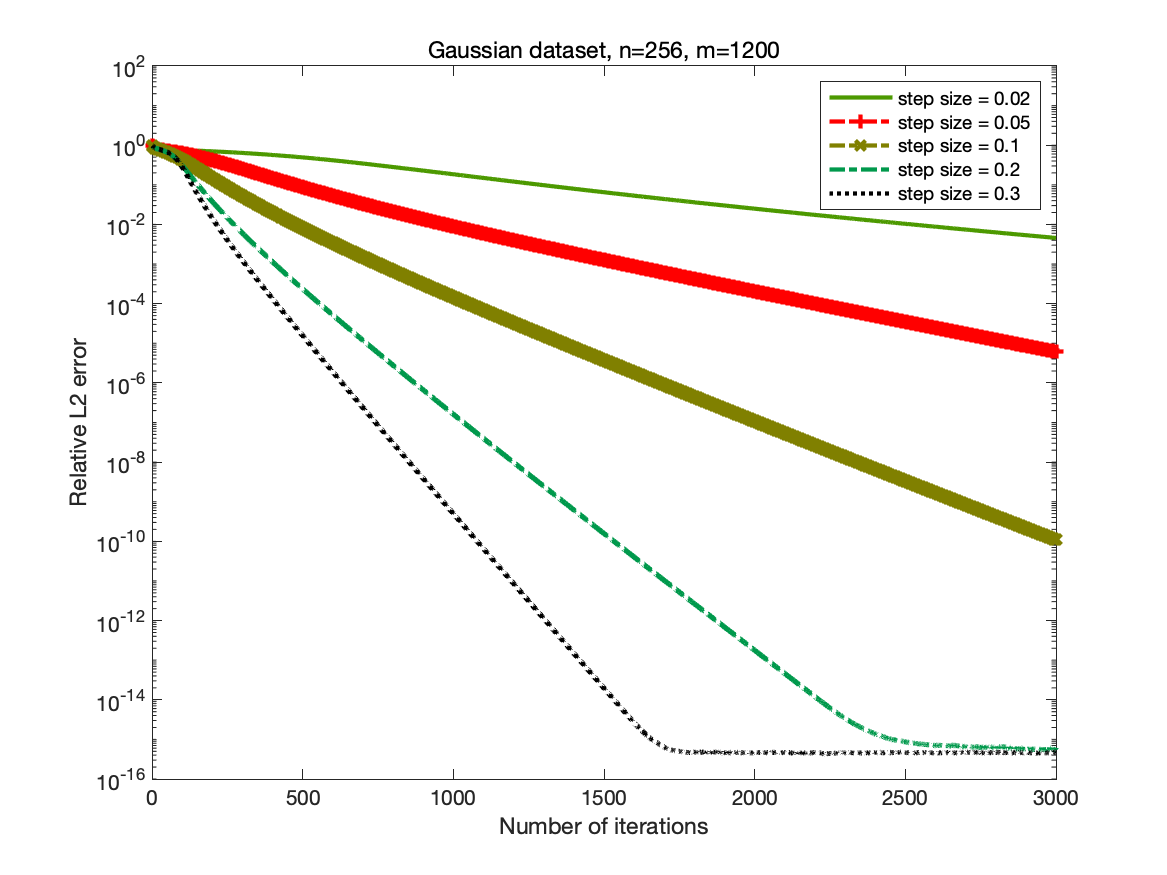
\includegraphics[width=1\linewidth]{./fig/gaussian+32.png}
			\caption{$m=800$}
		\end{minipage}
		\begin{minipage}{0.33\linewidth}
			\centering
			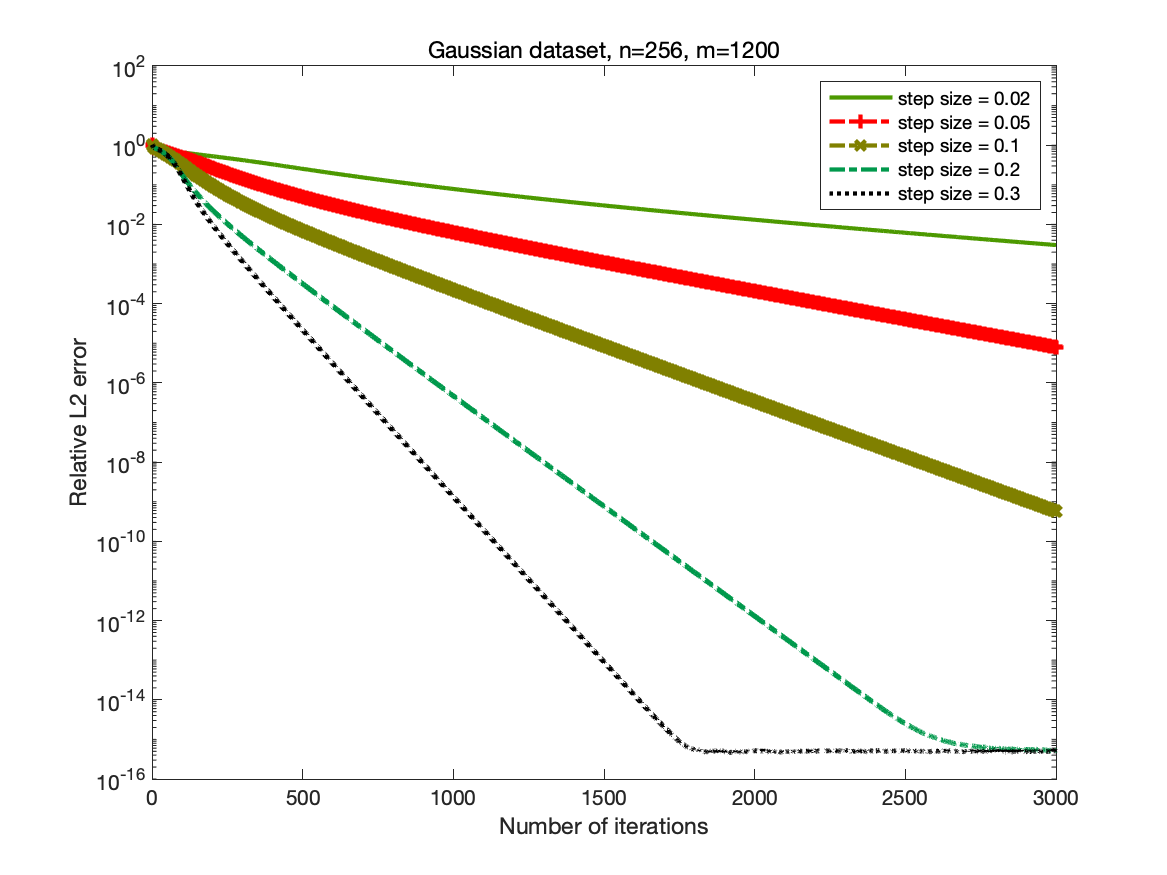
\includegraphics[width=1\linewidth]{./fig/gaussian+33.png}
			\caption{$m=1200$}
		\end{minipage}
		\caption*{Results on Gaussian dataset when $n=256$}
	\end{figure}
	\begin{table}
		\centering
		\begin{tabular}{|c|c|c|c|c|c|}
		\hline
		\multirow{2}{*}{ $\mu$} &\multicolumn{5}{c|}{$n = 128 $}\\\cline{2-6}
		 &$0.02$ &$0.05$ &$0.1$ &$0.2$ &$0.3$\\\hline
		$L=3$ & $4.33e-01$ & $9.37e-02$ & $5.57e-03$ & $5.65e-05$ & $7.22e-07$\\\hline
		$L=6$ & $6.09e-01$ & $5.52e-01$ & $3.87e-01$ & $1.48e-03$ & $5.11e-02$\\\hline
		$L=12$ & $1.89e-01$ & $1.42e-02$ & $7.40e-04$ & $4.44e-06$ & $1.22e-01$\\\hline
		\multirow{2}{*}{ $\mu$} &\multicolumn{5}{c|}{$n = 256 $}\\\cline{2-6}
 &$0.02$ &$0.05$ &$0.1$ &$0.2$ &$0.3$\\\hline
$L=3$ & $2.04e-04$ & $7.76e-09$ & $2.88e-15$ & $5.29e-16$ & $2.87e-16$\\\hline
$L=6$ & $1.43e-04$ & $6.87e-09$ & $2.83e-15$ & $3.98e-16$ & $2.88e-16$\\\hline
$L=12$ & $1.22e-04$ & $5.21e-09$ & $2.71e-15$ & $3.21e-16$ & $2.77e-16$\\\hline
\multirow{2}{*}{ $\mu$} &\multicolumn{5}{c|}{$n = 512 $}\\\cline{2-6}
 &$0.02$ &$0.05$ &$0.1$ &$0.2$ &$0.3$\\\hline
$L=3$ & $3.14e-08$ & $3.25e-15$ & $1.09e-15$ & $3.47e-16$ & $2.08e-16$\\\hline
$L=6$ & $2.33e-08$ & $3.12e-15$ & $1.04e-15$ & $3.20e-16$ & $2.28e-16$\\\hline
$L=12$ & $4.56e-08$ & $3.36e-15$ & $1.16e-15$ & $3.28e-16$ & $2.30e-16$\\\hline
		\end{tabular}
		\caption{Relative error after $3000$ iterations by Wirtinger Flow on dataset CDP\label{CDP}}
		\end{table}
\begin{figure}
	\begin{minipage}{0.33\linewidth}
		\centering
		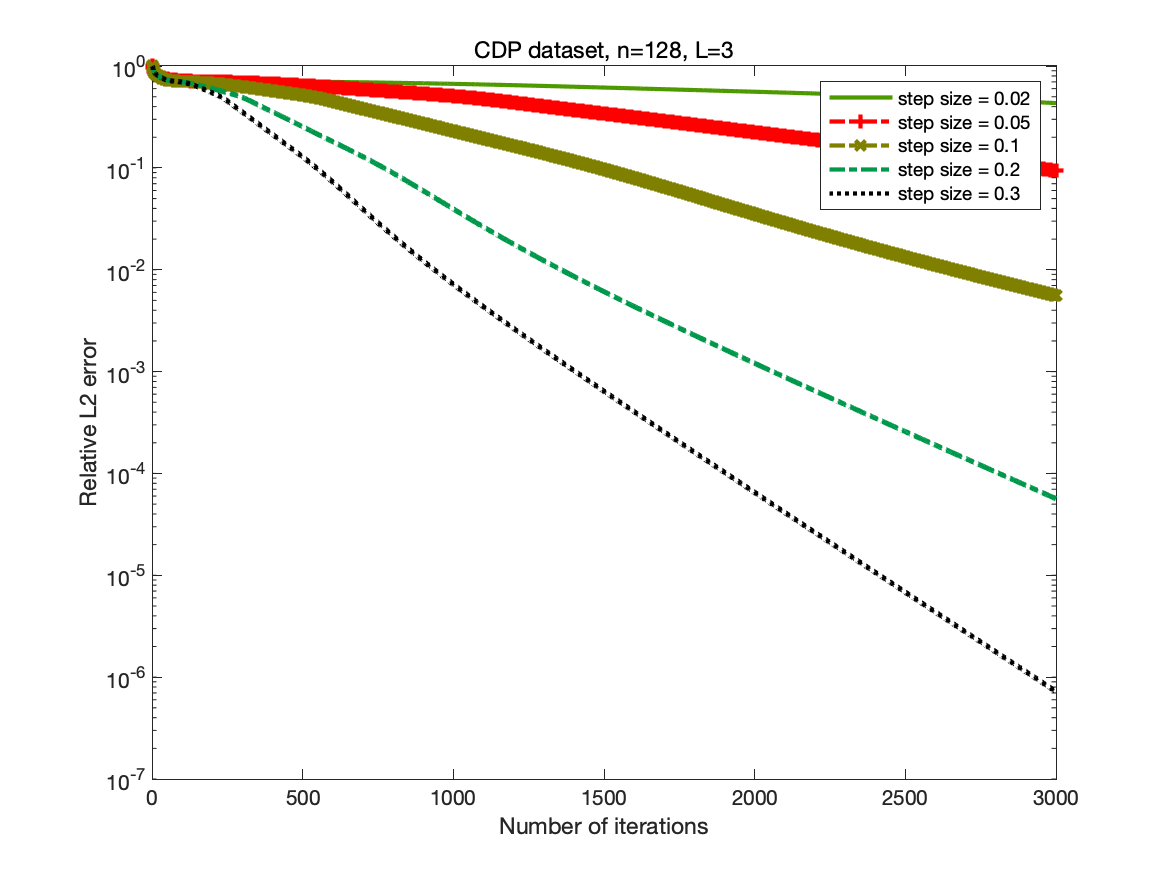
\includegraphics[width=1\linewidth]{./fig/CDP+11.png}
		\caption{$L=3$}
	\end{minipage}
	\begin{minipage}{0.33\linewidth}
		\centering
		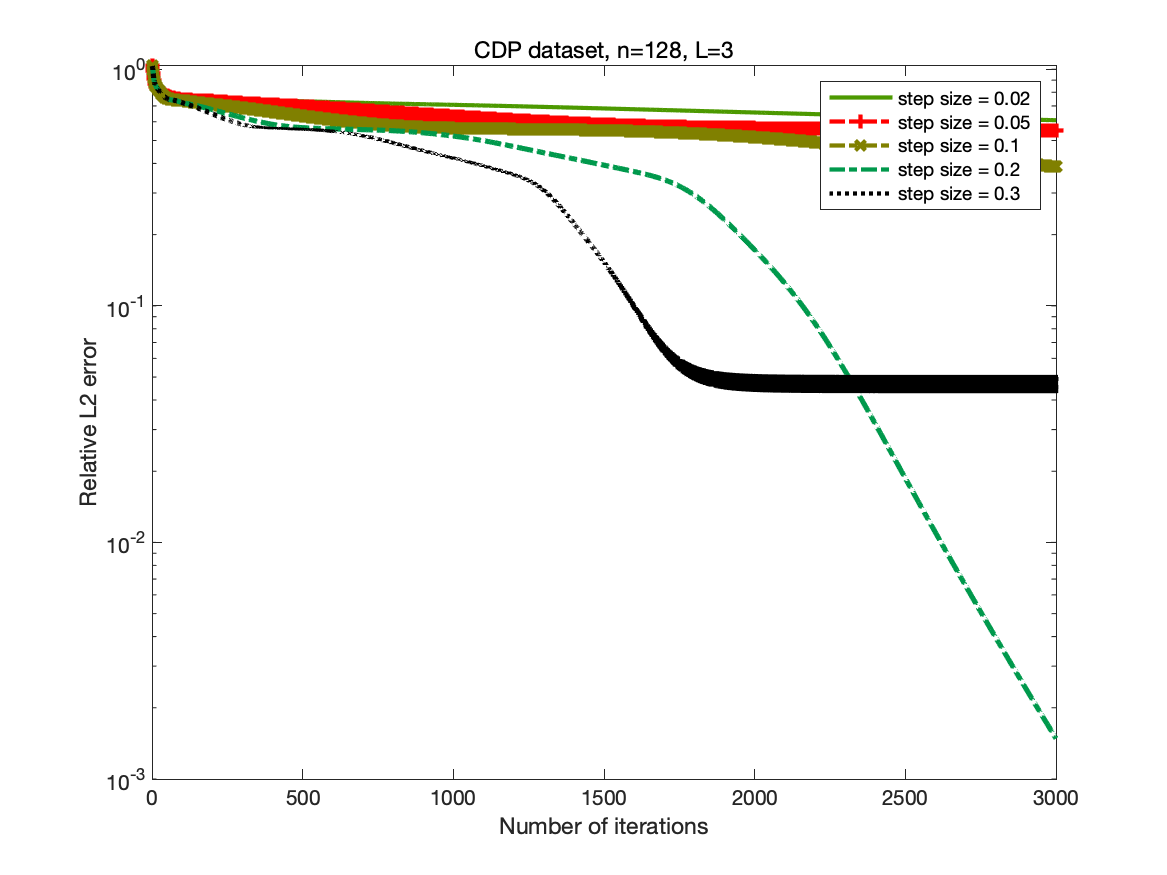
\includegraphics[width=1\linewidth]{./fig/CDP+12.png}
		\caption{$L=6$}
	\end{minipage}
	\begin{minipage}{0.33\linewidth}
		\centering
		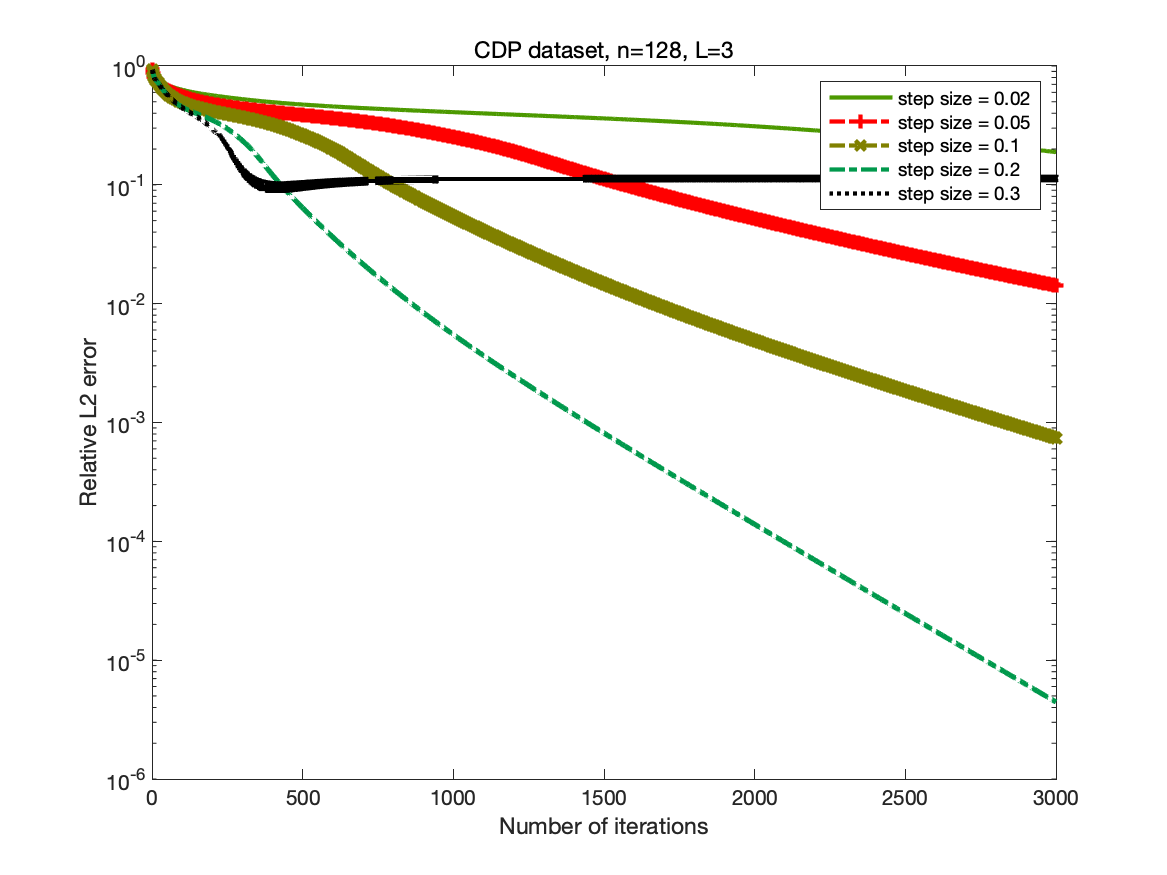
\includegraphics[width=1\linewidth]{./fig/CDP+13.png}
		\caption{$L=12$}
	\end{minipage}
	\caption*{Results on CDP dataset when $n=128$}
\end{figure}
\begin{figure}
	\begin{minipage}{0.33\linewidth}
		\centering
		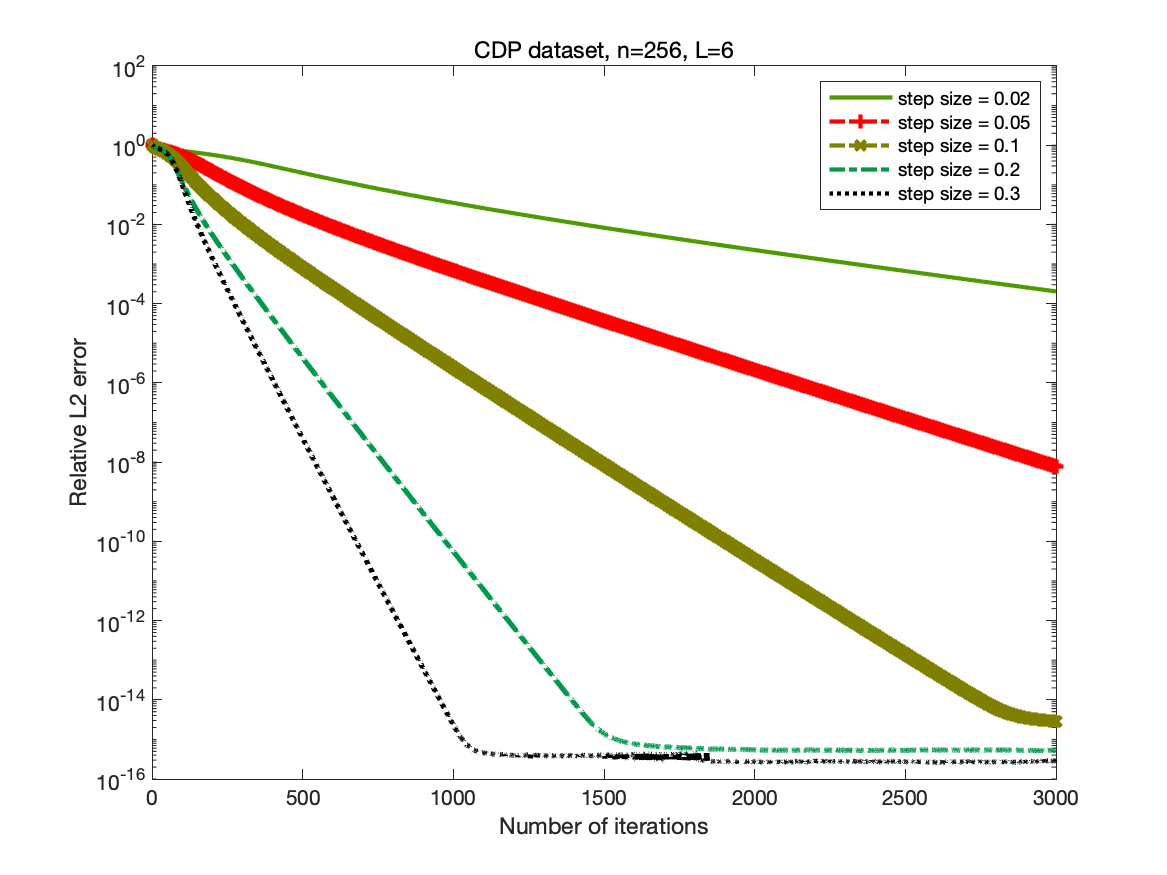
\includegraphics[width=1\linewidth]{./fig/CDP+21.png}
		\caption{$L=3$}
	\end{minipage}
	\begin{minipage}{0.33\linewidth}
		\centering
		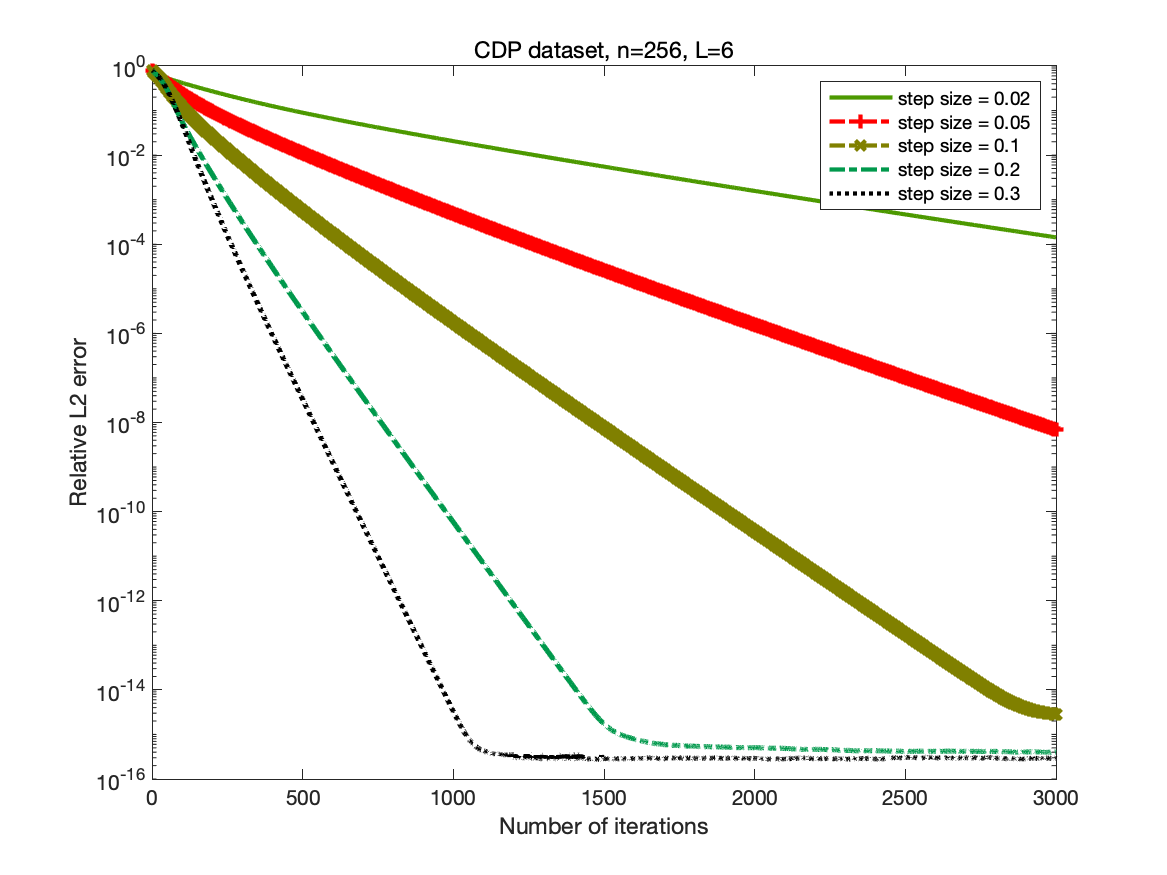
\includegraphics[width=1\linewidth]{./fig/CDP+22.png}
		\caption{$L=6$}
	\end{minipage}
	\begin{minipage}{0.33\linewidth}
		\centering
		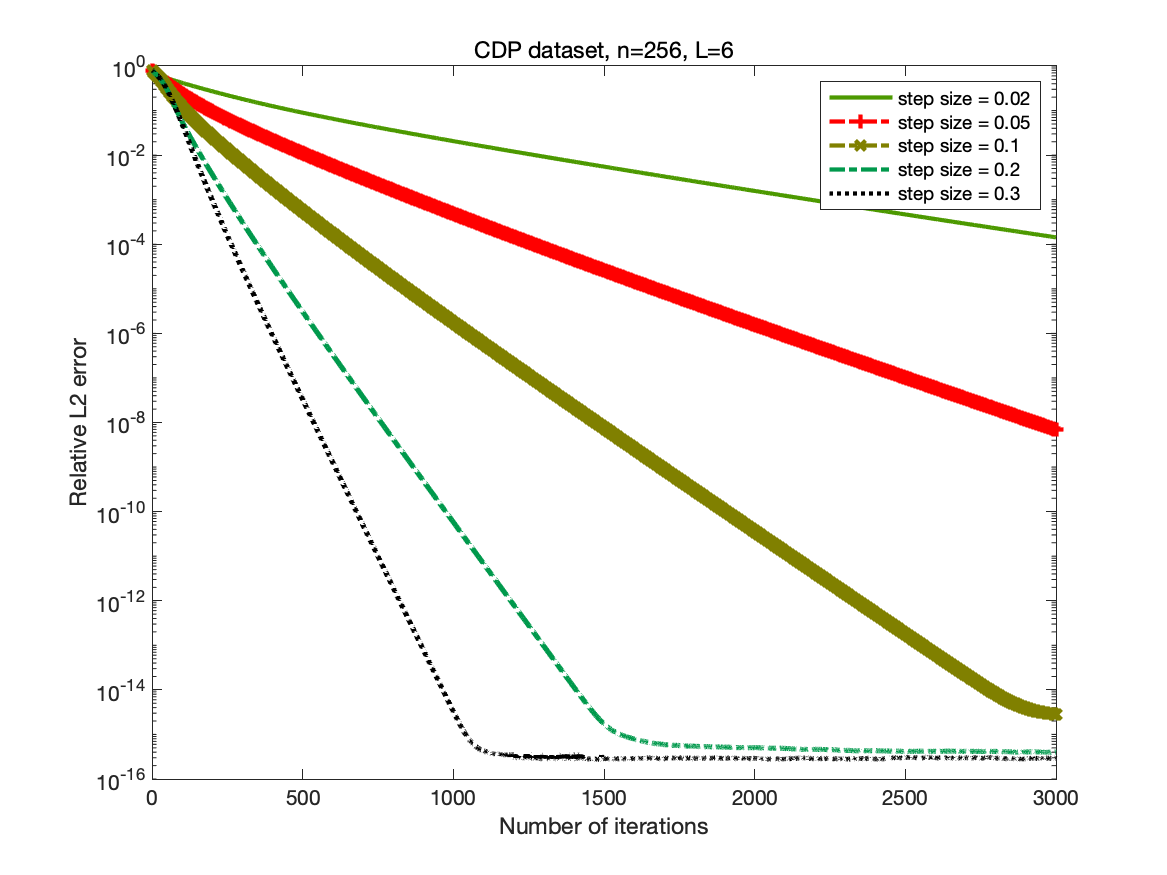
\includegraphics[width=1\linewidth]{./fig/CDP+22.png}
		\caption{$L=12$}
	\end{minipage}
	\caption*{Results on CDP dataset when $n=256$}
\end{figure}
\begin{figure}
	\begin{minipage}{0.33\linewidth}
		\centering
		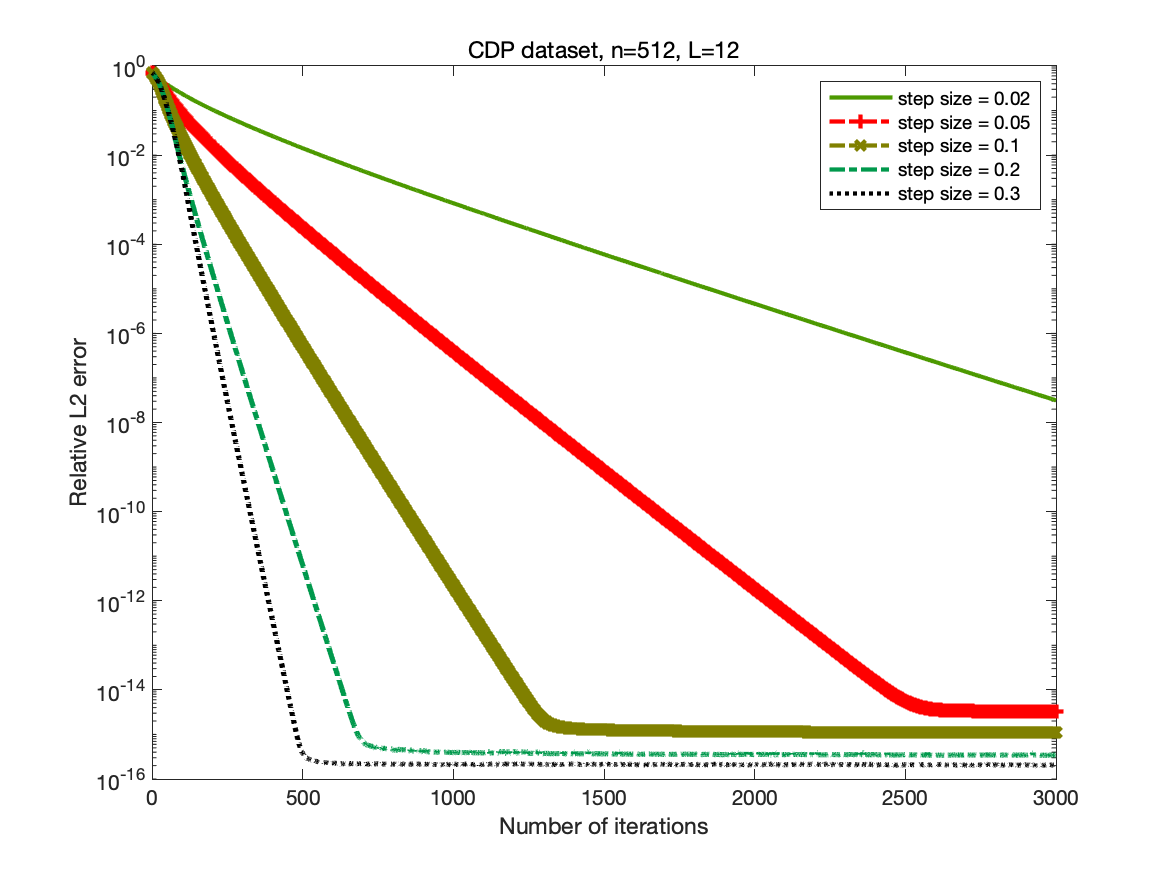
\includegraphics[width=1\linewidth]{./fig/CDP+31.png}
		\caption{$L=3$}
	\end{minipage}
	\begin{minipage}{0.33\linewidth}
		\centering
		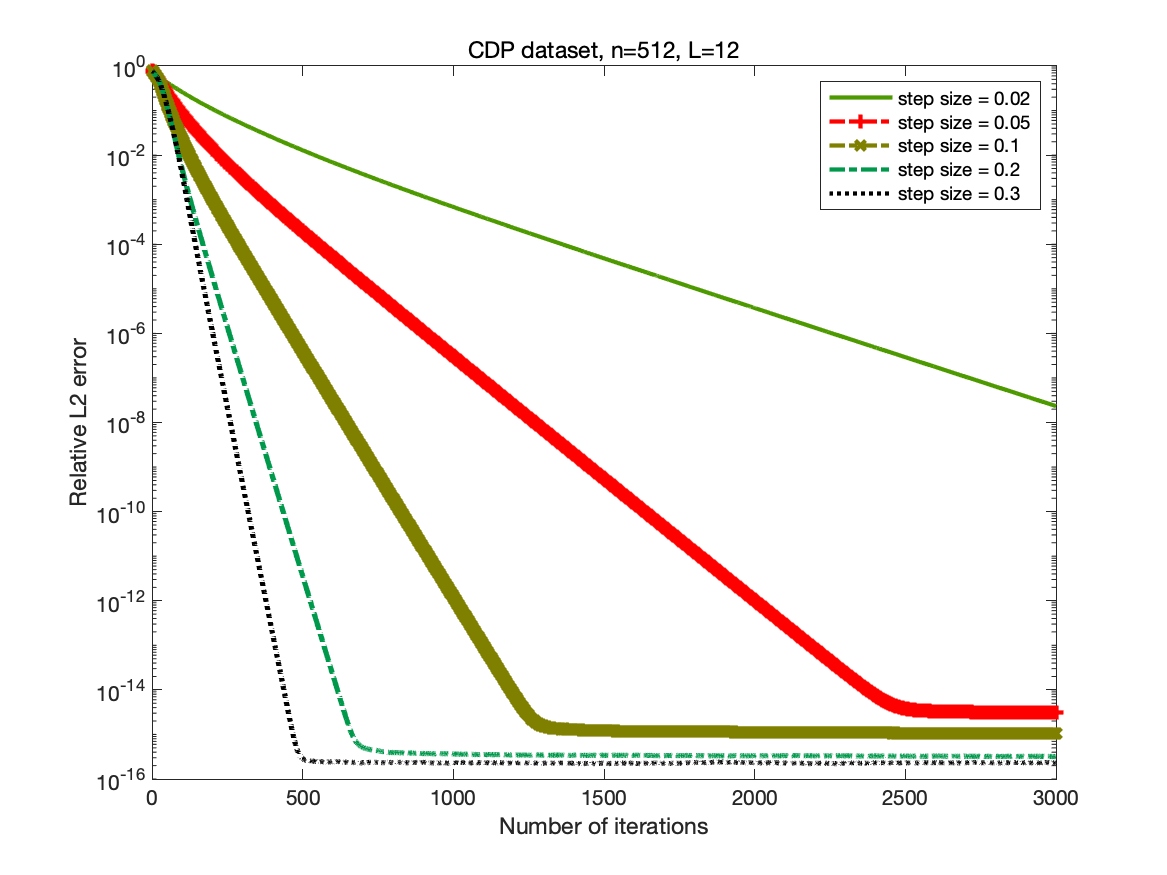
\includegraphics[width=1\linewidth]{./fig/CDP+32.png}
		\caption{$L=6$}
	\end{minipage}
	\begin{minipage}{0.33\linewidth}
		\centering
		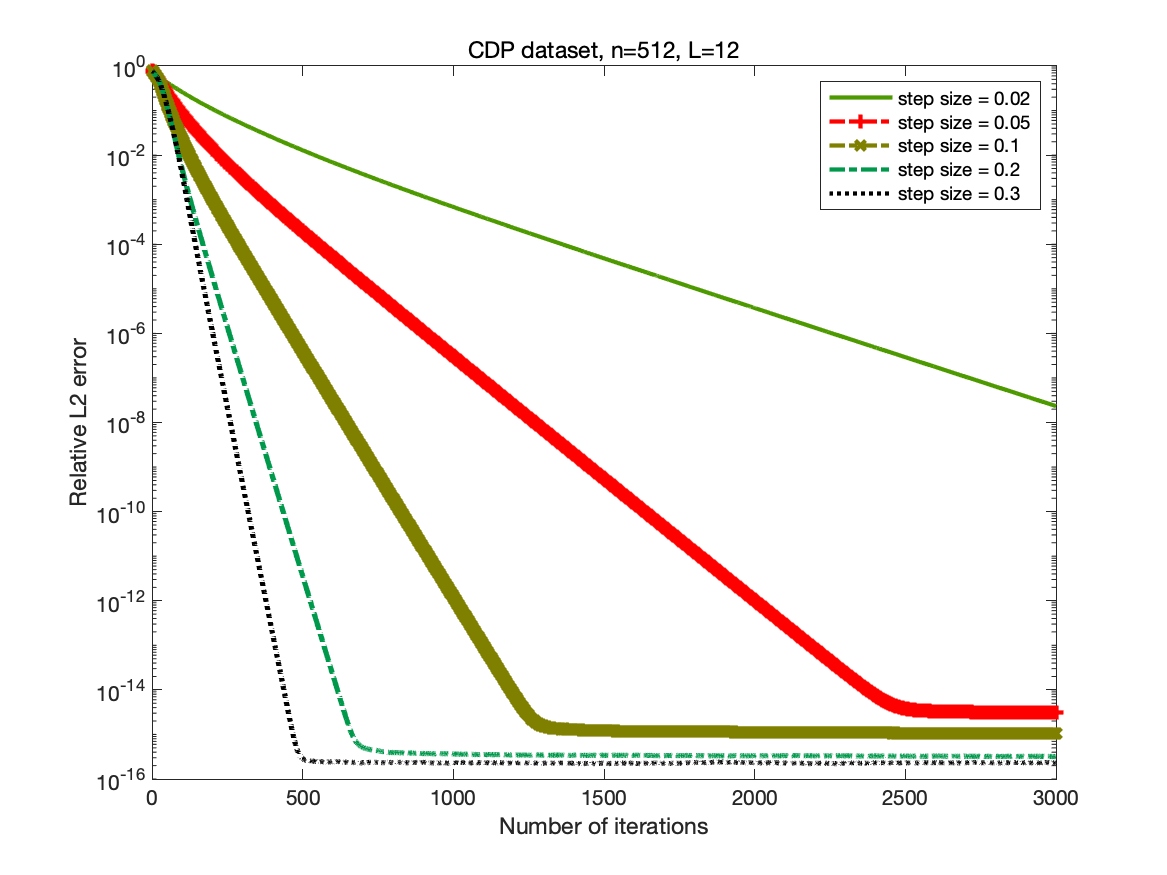
\includegraphics[width=1\linewidth]{./fig/CDP+32.png}
		\caption{$L=12$}
	\end{minipage}
	\caption*{Results on CDP dataset when $n=512$}
\end{figure}

Observation of the results tells that if the dataset is too small, i.e., $m$ is small, the iteration can converge to different restoration of the primitive data, which can be interpreted by the over-determined system of MSE problem. \cite{candes2015phase} has proved that Wirtinger Flow converges with high probability when $m\ge c_0n\log n$, where $c_0$ is a constant. On the other hand, $z\to |Az|$ is injective when $m=4n$. Such theorems suggest that large $m$ is required to gurantee the restoration of primitive data. However, it is helpful for restoration by setting the stepsize smaller.Secondly, given that the iterates finally converge to the primitive data, larger step size results in faster convergence. Anyway, our implementation of Wirtinger Flow attains very good results both in speed and accuracy.


\nocite{*}
\bibliographystyle{plain}  
\bibliography{ref}
\end{document}